\section{Use Cases}

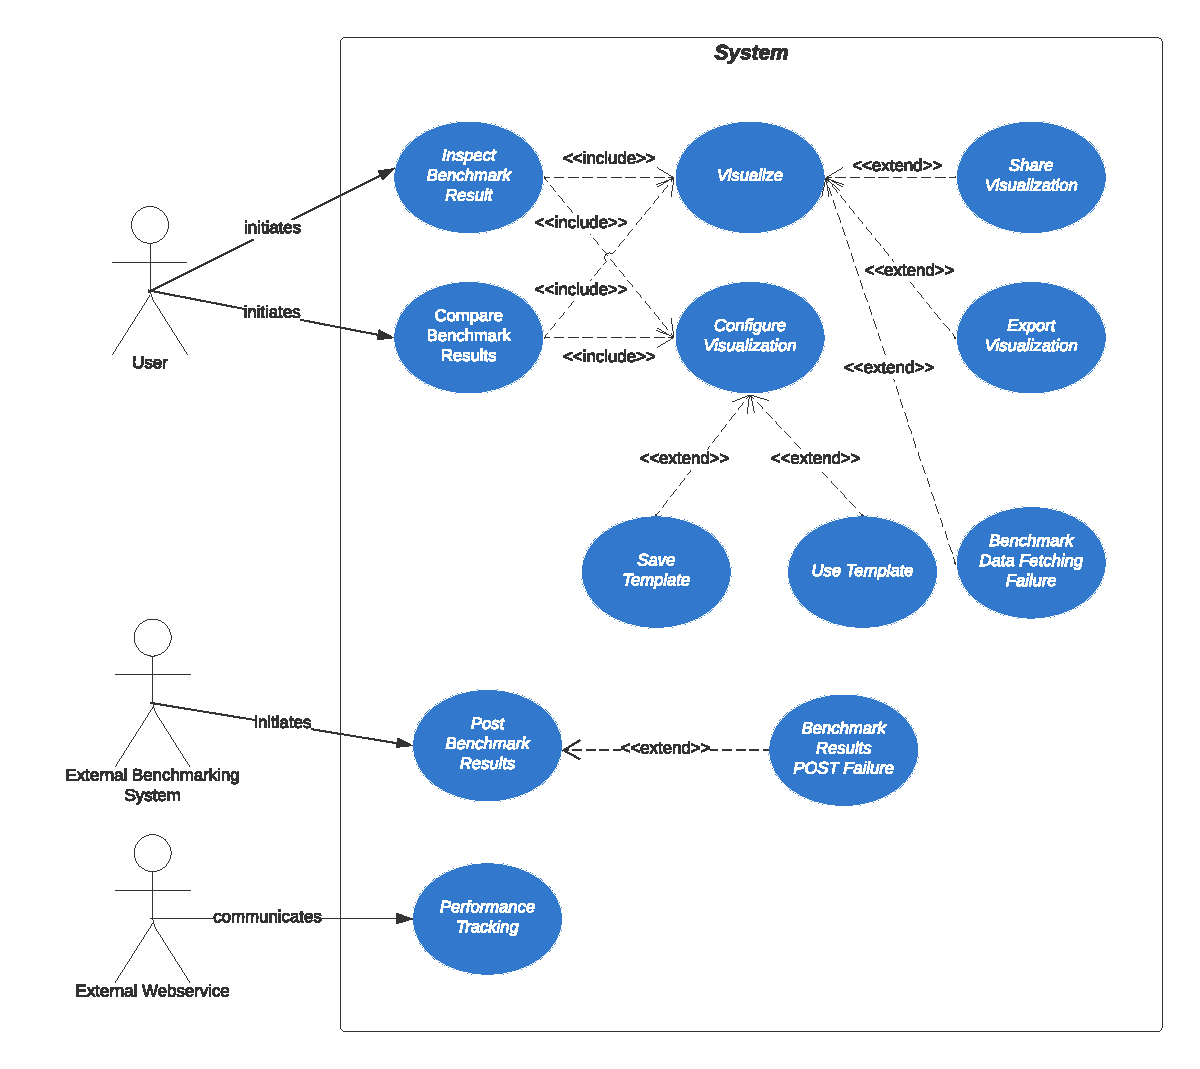
\includegraphics[width=\textwidth]{usecase.pdf}
\captionof{figure}{Use case diagram}

\case{Visualize}{cse:visualize}
{initiated by User}
{\gls{configuration} is available}
{\begin{enumerate}
    \item The web app sends a request to the backend containing the \gls{configuration}.
    \item The backend fetches the specified data from a databank.
    \item The backend does the calculations specified in the \gls{configuration} (mean, median, standard deviation).
    \item The backend sends the data back to the webapp.
    \item The webapp takes the data and generates the plot specified in the \gls{configuration}.
    \item The user gets redirected to a new site where he can inspect the generated plot.
\end{enumerate}}
{The plot specified by the \gls{configuration} gets shown to the User.}
{Shouldn't take more than 10 seconds}
\implementedby{scn:inspect_last_change}{cse:visualize}
\implementedby{scn:comp_benchmarks}{cse:visualize}

\bigskip

\case{Configure Visualization}{cse:config_vis}
{initated by User}
{User selected the \enquote{Create New Plot} option}
{\begin{enumerate}
    \item A popup appears.
    \item The user chooses a plot type.
    \item The user chooses between certain options that are specific to the plot type.
\end{enumerate}}
{A \gls{configuration} gets created.}
{The available options should be understandable without any previous knowledge or otherwise described by a short text.}
\implementedby{scn:inspect_last_change}{cse:config_vis}
\implementedby{scn:comp_benchmarks}{cse:config_vis}

\bigskip

\case{Inspect Change}{cse:inspect_change}
{initated by User}
{benchmark data for change is available}
{\begin{enumerate}
    \item The user selects a single change.
    \item The user initiates the \texttt{Configure Visualization} use case by selecting the \enquote{Create New Plot} option.
    \item Once the user is satisfied with his \gls{configuration}, he initiates the \texttt{Visualize} use case by selecting the \enquote{Create New Plot} option in the popup.
\end{enumerate}}
{Visualization is displayed to the user}
{???}
\implementedby{scn:inspect_last_change}{cse:inspect_change}

\bigskip

\case{Compare Benchmark Data}{cse:comp_data}
{intiated by User}
{benchmark results for all selected change are available}
{\begin{enumerate}
    \item The user selects multiple changes.
    \item The user initiates the \texttt{Configure Visualization} use case by selecting the \enquote{Create New Plot} option.
    \item Once the user is satisfied with his \gls{configuration}, he initiates the \texttt{Visualize} use case by selecting the "Generate New Plot" option in the popup.
\end{enumerate}}
{Visualization is displayed to the user}
{???}
\implementedby{scn:comp_benchmarks}{cse:comp_data}

\bigskip

\case{Share Visualization}{cse:share_vis}
{initiated by User}
{A \gls{visualization} has been generated}
{\begin{enumerate}
    \item The user selects the \enquote{Share Visualization} option.
    \item A link gets displayed.
    \item The link redirects any visitors to the same \gls{visualization}.
\end{enumerate}} 
{A link is shown which redirects to the \gls{visualization}}
{???}
\implementedby{scn:inspect_last_change}{cse:share_vis}

\bigskip

\case{Export Visualization}{cse:export_vis}
{initiated by User}
{A \gls{visualization} has been generated}
{\begin{enumerate}
    \item The user selects the \enquote{Export Visualization} option.
    \item A popup appears.
    \item The user chooses a filetype for the export.
    \item The user confirmes and downloads the \gls{visualization} in the choosen file format.
\end{enumerate}} 
{The User is offered a download of an export of the \gls{visualization}}
{Support for the filetypes png, pdf and pgf (what is the preferred latex format?)}
\implementedby{scn:comp_benchmarks}{cse:export_vis}

\bigskip

\case{Save Template}{cse:save_template}
{initiated by User, (maybe web browser as well? the cookies get stored on the web browser)}
{The user is in the \texttt{Configure Visualization} use case}
{The \texttt{Save Template} use case extends the \texttt{Configure Visualization} use case.
\begin{enumerate}
    \item The User selects the \enquote{save template} option.
    \item The User enters a name for the \gls{template}.
    \item The webapp stores the template locally (cookies).
\end{enumerate}} 
{\Gls{template} is stored on the locally (might add global templates for later?)}
{Requires less than 1kB of memory}
\implementedby{scn:inspect_last_change}{cse:save_template}

\bigskip

\case{Use Template}{cse:use_temp}
{initiated by User (maybe web browser as well? the cookies get stored on the web browser)}
{The user is in the \texttt{Configure Visualization} use case and a \gls{template} is available locally}
{The \texttt{Use Template} use case extends the \texttt{Configure Visualization} use case.
\begin{enumerate}
    \item The User selects the \enquote{use template} option.
    \item User is shown a list of all available \glspl{template}.
    \item User selects a \gls{template} from the list.
    \item The current \gls{configuration} options get set to the values specified in the template.
\end{enumerate}} 
{The \gls{template} is applied to the current configuration.}
{???}
\implementedby{scn:comp_benchmarks}{cse:use_temp}

\bigskip

\case{Post Benchmark Results}{cse:post_benchmark_res}
{initiated by External Benchmarking System}
{The external benchmarking system ran the benchmarks}
{\begin{enumerate}
    \item The benchmarking system makes a POST request to the backend containing the new benchmark data in \acrshort{json} format.
    \item The backend converts the received data into the correct format.
    \item The backend stores the received data in a database.
\end{enumerate}} 
{The received performance data is stored in a database}
{???}
\implementedby{scn:perf_tracking}{cse:post_benchmark_res}

\bigskip

\case{Performance Tracking}{cse:perf_tracking}
{communicates with External Webservice}
{New benchmark data has been posted to the backend}
{\begin{enumerate}
    \item The backend evaluates the performance of the new benchmark data.
    \item The backend compares the performance of the new benchmark with the performance of the corresponding benchmark of the last change.
    \item The backend relays the results to a configured number of hooks.
    \item The hooks contact their external webservices according to how they have been configured.
\end{enumerate}}
{The server fires a POST Request to all webhook subscribers}
{}
\implementedby{scn:perf_tracking}{cse:perf_tracking}
\implementedby{scn:inspect_last_change}{cse:perf_tracking}

\bigskip

\case{Benchmark Results POST Failure}{cse:benchmark_res_post_fail}
{return error code to External Benchmarking System}
{}
{This use case extends the \texttt{Post Benchmark Results} use case if an error occurs.
\begin{enumerate}
    \item The backend identifies the error.
    \item The backend creates a response with the correct error code.
\end{enumerate}}
{}
{}

\bigskip

\case{Benchmark Data Fetching Failure}{cse:benchmark_data_fetch_fail}
{displays error to User}
{This use case extends the \texttt{Visualization} use case if an error occurs.}
{\begin{enumerate}
    \item The backend identifies the error.
    \item The backend creates a response with the correct error code.
    \item The webapp displays an error message.
\end{enumerate}}
{}
{}

\bigskip

\case{UseCaseTemplate}{cse:use_case_template}
{Actors}
{Entry cond.}
{\begin{enumerate}
    \item Flow 1
    \item Flow 2
\end{enumerate}} 
{Exit cond.}
{Quality Requirements(?)}
